\section{Evaluation Design}
\label{sec:design}

We ask whether making claims explicit changes what can be concluded, and how the audit rules behave against reference mechanisms and conventional workflows. Seven research questions organise the evaluation:
\textbf{RQ1} How often, and through which assumption, do declared alternatives reverse a \textsc{primary} conclusion?
\textbf{RQ2} Does attribution evidence establish necessity, and is inadmissible evidence refused?
\textbf{RQ3} Which workflow errors does the audit detect, compared with conventional workflows on the same measurements?
\textbf{RQ4} How do \textsc{primary} standings relate to reference labels that are not defined by the audited intervention?
\textbf{RQ5} Does concept validation separate decodability from use?
\textbf{RQ6} Are the central findings stable across independently trained checkpoints?
\textbf{RQ7} Can studies be re-executed and re-audited exactly, and what does the evidence layer cost?

\paragraph*{Setup}
Table~\ref{tab:setup} summarises models, sites, samples and configurations. Central held-out inputs are correctly classified inputs drawn in seeded order after the development samples, so all central results are conditional on correct prediction. We test necessity and sufficiency of IG, gradient and random top-$k$ selections against the predicted-class margin.

\paragraph*{Protocols and blinding}
Each original held-out round had a plan frozen before it ran (Phase~7.5 and~7.75 plans in the repository). Later protocol revisions (ADR-053 on eligibility and ADR-054 on attainability) were informed by earlier results, so the work is not uniformly blind: the central 47/52 is a re-audit of held-out samples whose earlier audit had given 49/52. Every experiment new to this paper (Stages~2--4) had a protocol committed before execution, stating hypotheses, units, budgets and stopping rules; one baseline implementation error found during execution is reported in Section~\ref{sec:res-cmp}.

\paragraph*{Units and statistics}
The observational unit is a (site, held-out sample) pair for central claims and a (component, input) instance for reference models. Counts are exact. Wilson and input-level bootstrap intervals are descriptive and unclustered: instances share components and programs, and samples share checkpoints. Between-checkpoint spread is reported directly (RQ6). No interval here quantifies uncertainty over new models.

\section{Results}
\label{sec:results}

\subsection{RQ1: Configuration Dependence, Decomposed}
\label{sec:res-config}

On the six central sites, IG necessity was \textsc{primary}-supported on 52 of 302 held-out samples, and on 47 of these at least one declared \textsc{alternative} configuration contradicted the \textsc{primary} result. The committed per-sample records store only role-by-outcome counts, and their recorded reversal axes merge \textsc{alternative} and \textsc{stress\_test} findings, so they cannot attribute reversals to assumptions. We therefore re-ran the frozen central design unchanged, exporting every tested configuration with its axis values. Using the frozen macOS checkpoints on a Linux x86-64 server, the re-run reproduced every per-sample standing, finding code and outcome profile of the frozen results (\ReproDiffs{} differences over all six sites and six claims).

Table~\ref{tab:decomp} and Fig.~\ref{fig:decomp} decompose the reversals. A configuration that keeps $k$ keeps the selected units, because the IG ranking does not depend on the replacement, null or threshold; a configuration that changes $k$ changes the claim's subject. Of the \TotRev{} reversed samples, \TotFixed{} were reversed by an alternative that keeps the selected units fixed, and \TotKOnly{} only by alternatives that change $k$. Changing only the replacement reversed \TotRepl{} samples and changing only the null (count- to magnitude-matched controls) \TotNull{}; no reversal required a combination of axes without a single-axis explanation. The halved threshold reversed none of the supported claims, as Proposition~\ref{prop:thr} requires. The split differs by model: on the CNN pixel site \CnnFixed{} of \CnnRev{} reversals hold the units fixed, whereas on BERT-tiny only \TinyFixed{} of \TinyRev{} do and \TinyKOnly{} arise only from a change of $k$. All reversed samples retain the standing \textsc{supported} with the qualifying finding \texttt{alternative\_reverses} (Proposition~\ref{prop:roles}).

These counts are conditional on the declared family (Proposition~\ref{prop:mono}) and are not instability rates. They separate two readings that the aggregate 47/52 conflated: dependence of a \emph{fixed} claim on the intervention or control rule, and dependence of the \emph{claim itself} on the selection size.

\begin{table}[t]
\centering
\caption{Decomposition of ALTERNATIVE reversals of PRIMARY-supported IG necessity claims (re-run of the frozen central design, held-out samples). \emph{Any}: $\ge 1$ ALTERNATIVE configuration contradicts. \emph{Fixed}: a contradicting ALTERNATIVE keeps $k$, hence the selected units. Single-axis columns: contradiction by a configuration that differs from PRIMARY only on that axis. \emph{$k$ only}: reversed only by configurations that change $k$. Counts per sample; samples are nested in four checkpoints.}
\label{tab:decomp}
\setlength{\tabcolsep}{2.6pt}
\footnotesize
\resizebox{\columnwidth}{!}{%
\begin{tabular}{lrrrrrrrrr}
\toprule
 & & & \multicolumn{2}{c}{reversed} & \multicolumn{4}{c}{single-axis reversal} & \\
\cmidrule(lr){4-5}\cmidrule(lr){6-9}
site & $n$ & sup. & any & fixed & repl. & null & thr. & $k$ & $k$ only \\
\midrule
MLP input & 51 & 8 & 7 & 3 & 3 & 1 & 0 & 5 & 4 \\
MLP hidden & 51 & 4 & 2 & 2 & 2 & 0 & 0 & 2 & 0 \\
CNN pixels & 60 & 14 & 13 & 10 & 9 & 7 & 0 & 7 & 3 \\
CNN relu2 & 60 & 1 & 1 & 1 & 1 & 0 & 0 & 1 & 0 \\
BERT-tiny & 40 & 14 & 13 & 3 & 0 & 3 & 0 & 11 & 10 \\
BERT-base & 40 & 11 & 11 & 4 & 4 & 1 & 0 & 10 & 7 \\
\midrule
Total & 302 & 52 & 47 & 23 & 19 & 12 & 0 & 36 & 24 \\
\midrule
\multicolumn{10}{l}{\emph{fresh, never-inspected samples (protocol P3)}} \\
CNN pixels & 60 & 19 & 19 & 16 & 10 & 12 & 0 & 15 & 3 \\
CNN relu2 & 60 & 2 & 2 & 1 & 1 & 0 & 0 & 1 & 1 \\
BERT-tiny & 40 & 9 & 6 & 1 & 0 & 1 & 0 & 4 & 5 \\
\bottomrule
\end{tabular}}
\end{table}


\begin{figure}[t]
\centering
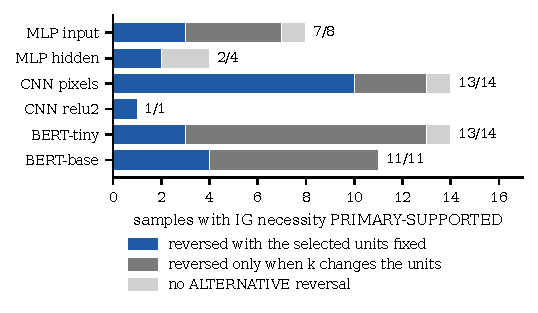
\includegraphics[width=\columnwidth]{figures/fig_decomposition.pdf}
\caption{ALTERNATIVE reversals of PRIMARY-supported IG necessity claims by source (re-run of the frozen design; Table~\ref{tab:decomp}). Counts per held-out sample.}
\label{fig:decomp}
\end{figure}

\subsection{RQ2: Attribution, Necessity and Admissibility}
\label{sec:res-adm}

On BERT-base, IG's \textsc{primary} selection contained \texttt{[SEP]} or \texttt{[CLS]} on 30 of 40 samples, and \texttt{[SEP]} on 10 of the 11 samples where necessity was supported. Declaring the claim the analyst usually intends, about the top-$k$ \emph{content} tokens with $k$, rankings and controls computed over content tokens only, gave 6 of 40 supports [0.07, 0.29]. Only 3 of the 11 all-token supports survived; 5 became \textsc{contradicted} and 3 \textsc{inconclusive} (a single content token leaves the control criterion unattainable), and 3 samples became newly supported. The special-token pattern was known from an earlier round before the content-token claim was declared. By the admissibility rule, attribution-only evidence never supported an intervention claim: all 2,480 attribution-only selection claims in this work (280 central, 1,960 InterpBench, 240 Tracr) were \textsc{unsupported} with \texttt{attribution\_is\_not\_intervention} (Proposition~\ref{prop:adm}). This is a consequence of the type rule, not empirical evidence that attribution is unreliable.

\subsection{RQ3: Comparison with Conventional Workflows}
\label{sec:res-cmp}

To test what the audit adds, we compared it with conventional workflows on \emph{identical} measurements: the frozen central evidence for 20 held-out MLP samples, logged as a careful researcher would (checkpoint and input hashes, configuration, drops, control drops, outcome). B0 reports the \textsc{primary} outcome; B1 adds \BOneLoc{} lines of checks written for this study (checkpoint, input, intervention present, controls present, $k$, outcome recomputation, and a multiverse rule); BeyondNN audits with the frozen plan (\PlanLoc{} lines, reused unchanged). We injected seven faults into both representations (Table~\ref{tab:cmp}). A first run used a baseline that ranked IG scores by signed rather than absolute value; after correcting it to the library's rule, the baseline and BeyondNN selected identical units and reached identical outcomes on 20 of 20 samples (largest drop difference $2.9\times10^{-6}$).

Single-configuration reporting surfaced none of the faults and would have reported 37 erroneous \textsc{supported} conclusions. The careful checker detected every fault, but only through a check written for that fault. The audit detected every fault from its declared plan without fault-specific code and with no false alert on unaffected samples. The two differed in two respects. B1's multiverse rule flagged one additional sample whose only contradicting alternative had an unattainable control criterion; the flat log records it as a contradiction, whereas the audit treats it as uninformative. And B1 localised tampered outcomes to the sample, whereas BeyondNN refused the whole evidence set because the edited record no longer matched its content hash. The result is therefore not that the audit detects errors a careful researcher cannot, but that its checks are part of the representation, apply to any plan, and encode edge cases (attainability, eligibility, provenance) that hand-written checks must anticipate. By lines of code it was not cheaper in this study.

\begin{table}[t]
\centering
\caption{Injected workflow faults on identical measurements (MLP, 20 held-out samples). Detected/affected, false alerts in parentheses. B0: single-configuration report. B1: conventional log with 54 lines of fault-specific checks. BeyondNN: the frozen plan, no fault-specific code. $^\ast$Study-level refusal: the edited trace fails its content hash and the evidence set is not loaded.}
\label{tab:cmp}
\setlength{\tabcolsep}{2.4pt}
\footnotesize
\resizebox{\columnwidth}{!}{%
\begin{tabular}{lrrrrr}
\toprule
fault & aff. & wrong sup. & B0 & B1 & BeyondNN \\
\midrule
F1 attribution as necessity & 20 & 20 & 0 & 20/20 (0) & 20/20 (0) \\
F2 wrong checkpoint & 5 & 1 & 0 & 5/5 (0) & 5/5 (0) \\
F3 wrong input & 5 & 0 & 0 & 5/5 (0) & 5/5 (0) \\
F4 wrong selection size & 5 & 1 & 0 & 5/5 (0) & 5/5 (0) \\
F5 omitted controls & 20 & 6 & 0 & 20/20 (0) & 20/20 (0) \\
F6 configuration dependence & 4 & 4 & 0 & 4/4 (1) & 4/4 (0) \\
F7 tampered outcome & 5 & 5 & 0 & 5/5 (0) & 5/5$^\ast$ (--) \\
\bottomrule
\end{tabular}}
\end{table}


\subsection{RQ4: Reference Labels Not Defined by the Audited Intervention}
\label{sec:res-ref}

\paragraph*{Compiled programs}
Eight held-out Tracr programs~\cite{lindner2023tracr} label each component by whether its variable is read by the output expression, independently of any intervention; the labels describe structural use, not per-input necessity. The \textsc{primary} resample test supported 0 of 400 decoy component--input tests (95\% Wilson upper bound 0.95\%), including 0 of 57 IG-selected decoy heads, and 591 of 760 tests of used components (77.8\% [74.7, 80.6]); each of the 19 used components passed on 28--38 of its 40 inputs and each of the 10 decoys on none. Two programs contain decoys correlated with the used variable: 0 of their 160 decoy tests were supported, of which 80 test an exact copy of the used variable. The 169 contradicted tests of used components are inputs on which the sampled counterfactual left the relevant value unchanged; an independent TransformerLens interchange agreed with the \textsc{primary} outcome on all 1,160 decisive instances. Mean replacement behaved similarly (0/400; 586/760), whereas zero replacement, a \textsc{stress\_test}, met the support rule for all 400 decoy and 760 used tests, because zero is not a valid one-hot value (Fig.~\ref{fig:reference}a).

\paragraph*{Trained transformers}
InterpBench's 18 held-out SIIT-trained transformers~\cite{gupta2024interpbench} were previously scored against labels filtered by the trained models' own resample ablations, which makes agreement partly circular. We re-scored the committed standings against \emph{specification} labels that use no intervention on the trained network: a node--input instance is necessary if the node is in the benchmark circuit and interchanging the corresponding node of the compiled high-level program changes that program's output. The \textsc{primary} test supported \IbTp{} of \IbPos{} specification-necessary instances and \IbFp{} of \IbNeg{} specification-unnecessary instances (\IbFpPct\%); zero replacement supported \IbZeroFp{} (\IbZeroFpPct\%) of the latter (Fig.~\ref{fig:reference}b). All \IbFp{} disagreements are non-circuit nodes, 17 of them in one model, on which the trained network's own resample ablation flips its prediction: the network does not implement its specification exactly there, and the audit reports the network, not the specification. This re-analysis was performed after the earlier results were known, and SIIT training itself uses interchange interventions, so the labels are independent of the audited evaluation but not of the intervention family that shaped the networks.

\begin{figure}[t]
\centering
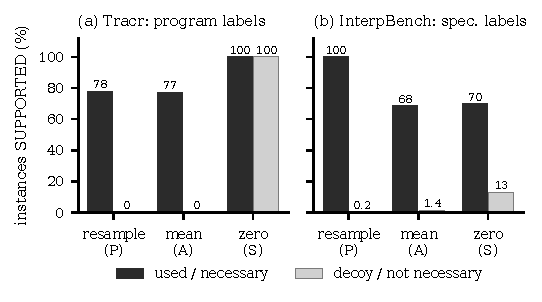
\includegraphics[width=\columnwidth]{figures/fig_reference.pdf}
\caption{Each configuration evaluated as if it were the only one, against reference labels not defined by the audited intervention: (a) program-defined structural labels of 8 compiled Tracr programs; (b) specification labels of 18 SIIT-trained InterpBench transformers. Percentages of instances supported; unclustered.}
\label{fig:reference}
\end{figure}

\subsection{RQ5: Decodability versus Use}

Four held-out numeric Tracr programs each contain a used indicator (K+), a decoy indicator read with coefficient exactly zero (K$-$) and a permuted-label control (K0). The encoding test supported K$-$ in all four programs, so decodability did not separate the variables; the use test did. Removing the K+ direction changed the target by 0.16--0.30, above the declared scale-relative minimum (0.2 standard deviations of the training target, ADR-055), and removing K$-$ changed it by exactly zero. All 4 K+ concepts were validated and none of the 8 K$-$ or K0 concepts under either threshold rule. The held-out programs did not discriminate between the scale-relative and an absolute threshold; on a constructed grid (6 use weights $\times$ 5 output scales) the absolute rule changed its verdict with the output scale in both directions while the relative rule validated exactly the weights $\ge 0.5$ at every scale. The relative rule was adopted after an absolute rule had failed to validate a known-used Tracr variable (use effect 0.06 against 0.1); no concept in a trained network has independent truth here.

\subsection{RQ6: Independently Trained Checkpoints}
\label{sec:res-seeds}

All central findings above rest on one checkpoint per model. We retrained the MLP and CNN with five seeds and re-ran the full central design on each checkpoint's held-out samples (Table~\ref{tab:seeds}, Fig.~\ref{fig:seeds}). Two hypotheses stated before the runs held on every checkpoint and site: IG necessity support exceeded random-selection support, and wherever at least three IG claims were supported, at least half carried an \textsc{alternative} reversal (75--100\%). The fixed-subject share replicated on the CNN pixel site (10--15 of 12--22 supports, 60--83\%). Absolute counts varied: IG supports on CNN pixels ranged from 12 to 22 of 60, so a single-checkpoint count is not a stable model-class estimate. On the CNN relu2 site, every IG necessity test carried \texttt{control\_criterion\_unattainable} on every checkpoint, so its few supports come from the remaining decisive tests. Gradient top-$k$ was supported on 37--41 of 60 CNN pixel samples on every checkpoint, against 12--22 for IG. The same code and seed produced different checkpoint digests on Linux and macOS; on these checkpoints the central counts were nevertheless identical. The BERT models have one checkpoint each.

\begin{table}[t]
\centering
\caption{Independently trained checkpoints (Linux x86-64; seeds 0--4) and the frozen macOS checkpoint. Each cell: IG necessity PRIMARY-supported / of which ALTERNATIVE-reversed / random selection supported, out of 51 (MLP) or 60 (CNN) held-out samples drawn by the same rule per checkpoint.}
\label{tab:seeds}
\setlength{\tabcolsep}{2.2pt}
\footnotesize
\resizebox{\columnwidth}{!}{%
\begin{tabular}{lcccccc}
\toprule
site & frozen & seed 0 & seed 1 & seed 2 & seed 3 & seed 4 \\
\midrule
MLP input & 8/7/1 & 8/7/1 & 8/8/0 & 7/6/0 & 4/4/1 & 7/6/1 \\
MLP hidden & 4/2/0 & 4/2/0 & 2/1/0 & 2/2/0 & 2/2/0 & 2/2/0 \\
CNN pixels & 14/13/1 & 14/13/1 & 22/20/2 & 20/19/3 & 17/16/0 & 12/12/1 \\
CNN relu2 & 1/1/0 & 1/1/0 & 2/1/1 & 3/3/1 & 4/3/0 & 4/3/0 \\
\bottomrule
\end{tabular}}
\end{table}


\begin{figure}[t]
\centering
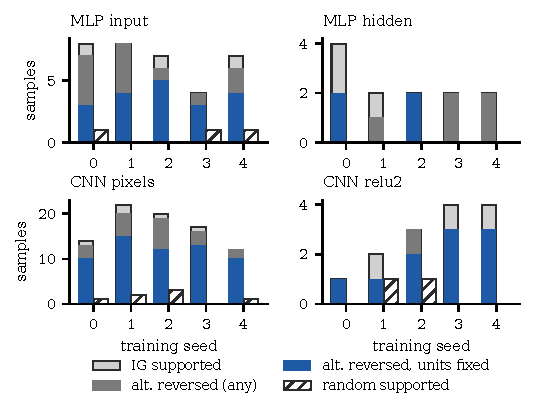
\includegraphics[width=\columnwidth]{figures/fig_seeds.pdf}
\caption{Central findings on five independently trained checkpoints per model (Table~\ref{tab:seeds}). Held-out sets are drawn by the same rule per checkpoint and differ between checkpoints.}
\label{fig:seeds}
\end{figure}

\subsection{RQ7: Re-execution, Re-audit and Cost}
\label{sec:res-repro}

\paragraph*{Re-execution}
Re-running the frozen central design from source on a different platform reproduced every per-sample audit output of the four central models (RQ1). For the MLP, evidence saved to disk (1.7 and 2.0~GB per site), reloaded in the same run and re-audited gave reports identical to the in-memory ones, and \texttt{verify\_report} re-derived each saved report from disk. Every tampered trace was refused on load (RQ3).

\paragraph*{Cost}
Table~\ref{tab:cost} and Fig.~\ref{fig:cost} separate evidence generation from the model-free audit. The audit and its verification are independent of the model, so their share falls as models grow: about a third of the total for the MLP and CNN sites and a few percent for the BERT models. At the level of one test, the evidence layer is not free: one \textsc{primary} IG necessity test with 50 controls on the 30-feature MLP took \CostBnnMs{}~ms through BeyondNN and \CostPlainMs{}~ms in plain PyTorch with Captum, about \CostRatio{} times longer, because record construction, hashing and provenance dominate the computation of so small a model. Saved evidence is large when every control effect is retained (33--39~MB per MLP sample).

\begin{table}[t]
\centering
\caption{Cost per held-out sample of the full central design (one CPU thread, Linux x86-64). Evidence: model execution and BeyondNN record construction for all results of the sample. Audit and verify: model-free. Share: audit + verify as \% of the total. Report: size of the site's report (MB). RSS: peak resident memory of one process (MB).}
\label{tab:cost}
\setlength{\tabcolsep}{2.2pt}
\footnotesize
\resizebox{\columnwidth}{!}{%
\begin{tabular}{lrrrrrrrr}
\toprule
site & $n$ & res. & evid. (s) & audit (s) & verify (s) & share & report & RSS \\
\midrule
MLP input & 51 & 72 & 3.7 & 0.967 & 1.154 & 36.7 & 20.3 & 5906 \\
MLP hidden & 51 & 72 & 4.4 & 1.033 & 1.206 & 33.7 & 20.0 & 6866 \\
CNN pixels & 60 & 72 & 3.7 & 1.132 & 1.181 & 38.8 & 23.9 & 3364 \\
CNN relu2 & 60 & 72 & 4.3 & 1.099 & 1.025 & 33.2 & 23.6 & 3836 \\
BERT-tiny & 40 & 69 & 70.4 & 1.211 & 1.105 & 3.2 & 15.4 & 1427 \\
\bottomrule
\end{tabular}}
\end{table}


\begin{figure}[t]
\centering
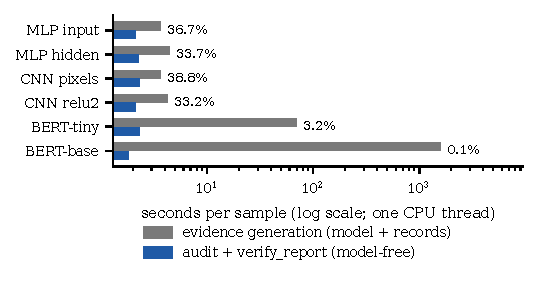
\includegraphics[width=\columnwidth]{figures/fig_cost.pdf}
\caption{Cost per held-out sample of the full central design: evidence generation (model execution and record construction) versus the model-free audit and verification; labels give the audit share. One CPU thread, Linux x86-64.}
\label{fig:cost}
\end{figure}

\subsection{Case Study: Plausibility versus Necessity on e-SNLI}

On 40 held-out e-SNLI samples~\cite{camburu2018esnli,bowman2015snli}, with BERT-base fine-tuned on SNLI, we compared three equal-size token selections: annotator~1's rationale, IG's top-$k$ and a random set, each tested for necessity with the \texttt{[MASK]} replacement and matched controls. IG overlapped more with the human rationale than random sets did (token F1 0.34 [0.26, 0.42]; IG minus random $+0.149$, Bonferroni 98.75\% [0.031, 0.270]), yet necessity was supported for the human rationale on 10, for IG on 7 and for random sets on 3 of 40 samples, opposite to the directional prediction; the paired IG-minus-human difference was $-0.075$ [$-0.225$, 0.075], so no population difference is established. On 17 of the 40 samples the model predicts the same label with an empty premise (empty-premise accuracy 0.456 against chance 1/3~\cite{gururangan2018artifacts}), and 5 of IG's 7 supports fall in that stratum (exploratory). Human rationales are plausibility references, not causal ground truth; one annotator, one model and 40 samples limit this study.
